
\documentclass[conference]{IEEEtran}
\usepackage[utf8]{inputenc}
\usepackage[english]{babel}
\usepackage{graphicx}
\usepackage{amsmath}
\usepackage{hyperref}
\usepackage{natbib}
\usepackage{geometry}
\usepackage{booktabs}
\usepackage{array}
\geometry{margin=1in}

\title{Deterministic Random Bit Generators NIST techniques comparison}
\author{
    Tomas Bedoya \\
    Daniel Andres Jaimes Cardenas \\
    Eder Leandro Carbonero Baquero \\
    \textit{Universidad de los Andes, Colombia}
}
\date{\today}

\begin{document}

\maketitle
\begin{abstract}
Aquí va el resumen del artículo, una breve descripción del problema, la metodología y los resultados.
\end{abstract}

\section{Introduction}
Due to the deterministic nature of traditional computers, which is what most people and appliances use to this day and will continue being so for the foreseeable future, Random Number Generation (RNG) has proven to be a challenge. Due to the reliance of cryptographic algorithms, communication protocols and other security systems in random values, there’s a constant race to find ever-better sources of randomness that follow the international standards of quality; the higher the randomness of a source, the greater the security it provides. This proves to be a challenge, however, for true randomness is difficult to find. Computers themselves cannot produce it and rely on Pseudo Random Number Generation (PRNG) to simulate random values. Other techniques, such as finding random measurements on certain like the time between user key strokes or mouse movements have proven to be unsatisfactory when put under statistical scrutiny (Mechalas, 2018). 
To guarantee that sensible processes utilize proper random sources, the NIST structured the SP 800-90 Standards for Random Number Generation (RNG) for safe RNG in cryptographic contexts. The following sections delve deep into several RNG methods, both of pseudo and true randomness, that follow these standards. They explore the different entropy sources they use (or don’t), analyses how they extract random number chains from them, and evaluate the quality of their randomness through a series of statistical evaluations. Our aim is to understand better where RNG stands today, to evaluate how they fare against each other, and determine which of these methods work better for which applications.


\section{General defintions}
\noindent
With the aim of providing a broader understanding of the various concepts addressed in this document, the following are definitions of some of the acronyms that will be mentioned throughout the text.
% genericos.tex

\begin{table}[h!]
\centering
\begin{tabular}{@{}ll@{}}
\toprule
\textbf{Acronym} & \textbf{Meaning} \\ \midrule
CTR\_DRBG & Counter mode Deterministic Random Bit Generator \\
NIST & National Institute of Standards and Technology \\
AES & Advanced Encryption Standard \\
RBG & Random Bit Generator \\
DRBG & Deterministic Random Bit Generator \\
PRNG & Pseudorandom Number Generator \\ \bottomrule
\end{tabular}
\caption{Acronyms definitions.}
\label{tab:acronyms}
\end{table}

\section{methodologies}
\section{Methology}
\subsection{Random Number Generation}
\label{sec:random_generation}

For this exercise, three different forms of random number generation were performed. The first was through the \textit{CTR\_DRBG} algorithm, which used random keys generated by the \texttt{random} function of the Python programming language version 3.9 as seeds and was executed on a MacBook Pro M3 Pro computer. This detail may lead to different results if the experiment is replicated. However, we assume that Python's \texttt{random} function generates a uniform randomness distribution, simulating an entropic system for generating random bits.

For the second option, a sequential range of seeds was chosen, which were formatted in 32 bits to ensure compatibility with AES encryption. The sequence started at 1 and increased by one until reaching 50 million seeds. These seeds were then used to execute the \textit{CTR\_DRBG} algorithm, which generates the pseudo-random bit values.

The third approach made use of the Beacon system. In this case, the official NIST API was consumed to retrieve the last 15,600 random bits, generated from 512-bit values, obtained from the historical records maintained by the system.


\section{techniques}
\section{CTR\_DRBG Counter mode Deterministic Random Bit Generator}
\label{sec:counter_mode_deterministic_random_bit_generator}

\begin{quote}
\textbf{CTR\_DRBG (Counter mode Deterministic Random Bit Generator)} is a standardized method for constructing a deterministic random bit generator (PRNG) using a block cipher operating in counter (CTR) mode. This technique is defined in NIST Special Publication 800-90A, titled \textit{``Recommendation for Random Number Generation Using Deterministic Random Bit Generators''}. Essentially, CTR\_DRBG transforms a secure symmetric cipher---such as AES---into a cryptographically strong source of pseudorandom bits. The counter mode ensures that each generated block is unique by systematically incrementing a counter value for each new data request, thus preventing the repetition of output sequences under the same key and seed. This approach is widely used in cryptographic applications requiring high security and reliability in random data generation, such as key generation, initialization vectors, and session tokens.
\end{quote}

\subsection*{How It Works}

The internal state of the CTR\_DRBG consists of two components:

\begin{itemize}
    \item \textnormal{\textbf{V}}: A state vector that acts as a counter.
    \item \textnormal{\textbf{Key}}: A symmetric encryption key (commonly 128 or 256 bits).
\end{itemize}

To generate random output, the algorithm encrypts sequential values derived from \texttt{V} using the current \texttt{Key}. For each block of output, the counter \texttt{V} is incremented. 

A secure seed—typically composed of entropy input, a nonce, and optional personalization string—is required to properly initialize the internal state.

\textit{CTR\_DRBG} utilizes an approved block cipher algorithm in counter (CTR) mode, as described in \cite{nist80090a}. Unlike the standard CTR mode, it allows the counter field to occupy only a portion of the cipher input block, as specified in \cite{nist80038d}.

For context, the block size depends on the cipher: 64 bits for TDEA and 128 bits for AES. The same block cipher algorithm and key length are used consistently throughout all encryption operations in the DRBG. These parameters must meet or exceed the required security level of the intended application.

The construction of \textit{CTR\_DRBG} revolves around an internal update function, \texttt{CTR\_DRBG\_Update}, illustrated in Figure~\ref{fig:ctr_drbg_update}. This function is invoked during instantiation, reseeding, and random bit generation to update the internal state using newly provided entropy or additional input. It also ensures that the internal state changes appropriately after every generation step.

Figure~\ref{fig:ctr_drbg_stages} outlines the full operation of \textit{CTR\_DRBG} in three stages: instantiation, generation, and reseeding.

\begin{figure}[htbp]
    \centering
    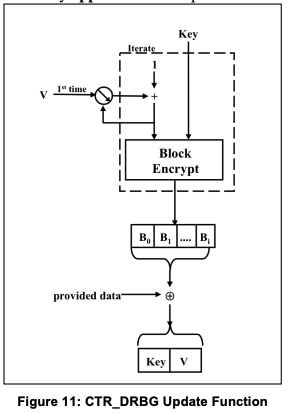
\includegraphics[width=0.9\linewidth]{images/Figure11_CTR_DRBG_Update_Function.png}
    \caption{CTR\_DRBG Update function as shown in \cite{nist80090a}.}
    \label{fig:ctr_drbg_update}
\end{figure}

\begin{figure}[htbp]
    \centering
    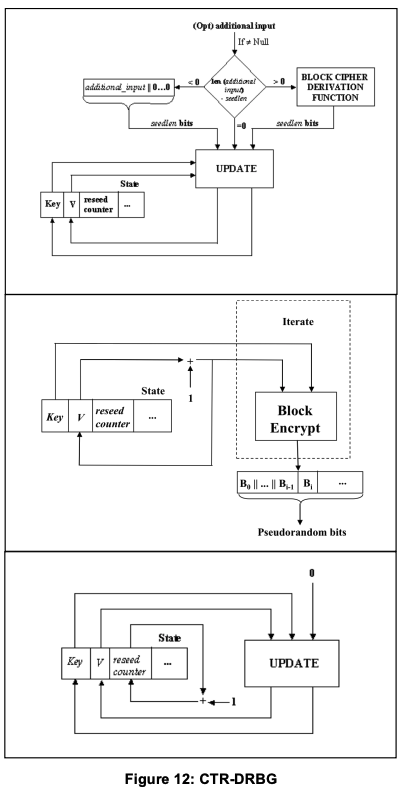
\includegraphics[width=0.9\linewidth]{images/Figure12_CTR_DRBG.png}
    \caption{The three stages of CTR\_DRBG operation as illustrated in \cite{nist80090a}.}
    \label{fig:ctr_drbg_stages}
\end{figure}

To provide an overview of what can be found in the source article, we can say that \textit{CTR\_DRBG} is a deterministic random bit generator that uses an approved symmetric encryption algorithm, such as AES, in counter (CTR) mode to produce secure random bits. Its internal state consists of a counter vector called \texttt{V} and a secret key, \texttt{Key}, which are updated through an internal function named \texttt{CTR\_DRBG\_Update} during instantiation, generation, and reseeding, thus ensuring the cryptographic security of the generator. At each step, \texttt{V} is encrypted with \texttt{Key} and incremented to generate non-repeating pseudorandom blocks. It requires a secure initial seed with sufficient entropy to avoid predictability and can be periodically reseeded to maintain long-term security. This flexible design allows for the use of variable block sizes and key lengths depending on the algorithm (e.g., 128 bits for AES) and meets robust cryptographic standards, making it reliable for applications that require secure random number generation.

\subsection{AES - Advanced Encryption Standard}
\label{sec:aes}
\begin{quote}
\textbf{AES (Advanced Encryption Standard)} is a symmetric encryption algorithm widely used across various applications for securing data. It was established by the National Institute of Standards and Technology (NIST) in 2001 as a replacement for the older Data Encryption Standard (DES). AES operates on fixed-size blocks of data (128 bits) and supports key sizes of 128, 192, or 256 bits, providing a high level of security against brute-force attacks. The algorithm employs a series of transformations, including substitution, permutation, and mixing, to encrypt plaintext into ciphertext and vice versa. Its efficiency and robustness have made it the de facto standard for encryption in many cryptographic protocols and systems.
\end{quote}


\section{Results}
\subsection{Histogram analysis}
\label{sec:histogram_analysis}

\subsection{Distribution of Random Bits Generated with Python Random Seeds}
\label{sec:distribution_python_seed}

The distribution results of each technique are separated by the method used to obtain the seed versus the technique used to distill and obtain the random big number, so we can observe different results for each case.

To view the distribution of values, distribution graphs were used, either standard or uniform, depending on the input data. In our experiments, uniform distributions were shown. 8-bit segments were taken, dividing the entire input data set into byte blocks, obtaining bytes from 0 to 255. This range of possibilities gives us a visual of how the results are distributed.

We begin with the first technique, which was the generation of 6.25 million 32-byte seeds that were used to generate 6.25 million random bytes, or 50 million random bits, using the \textit{CTR\_DRBG} technique. The graph we see below leads us to the conclusion that there is a uniform distribution of the results without pronounced peaks, which are a symptom of an effective system in generating random bits.

\begin{figure}[htbp]
    \centering
    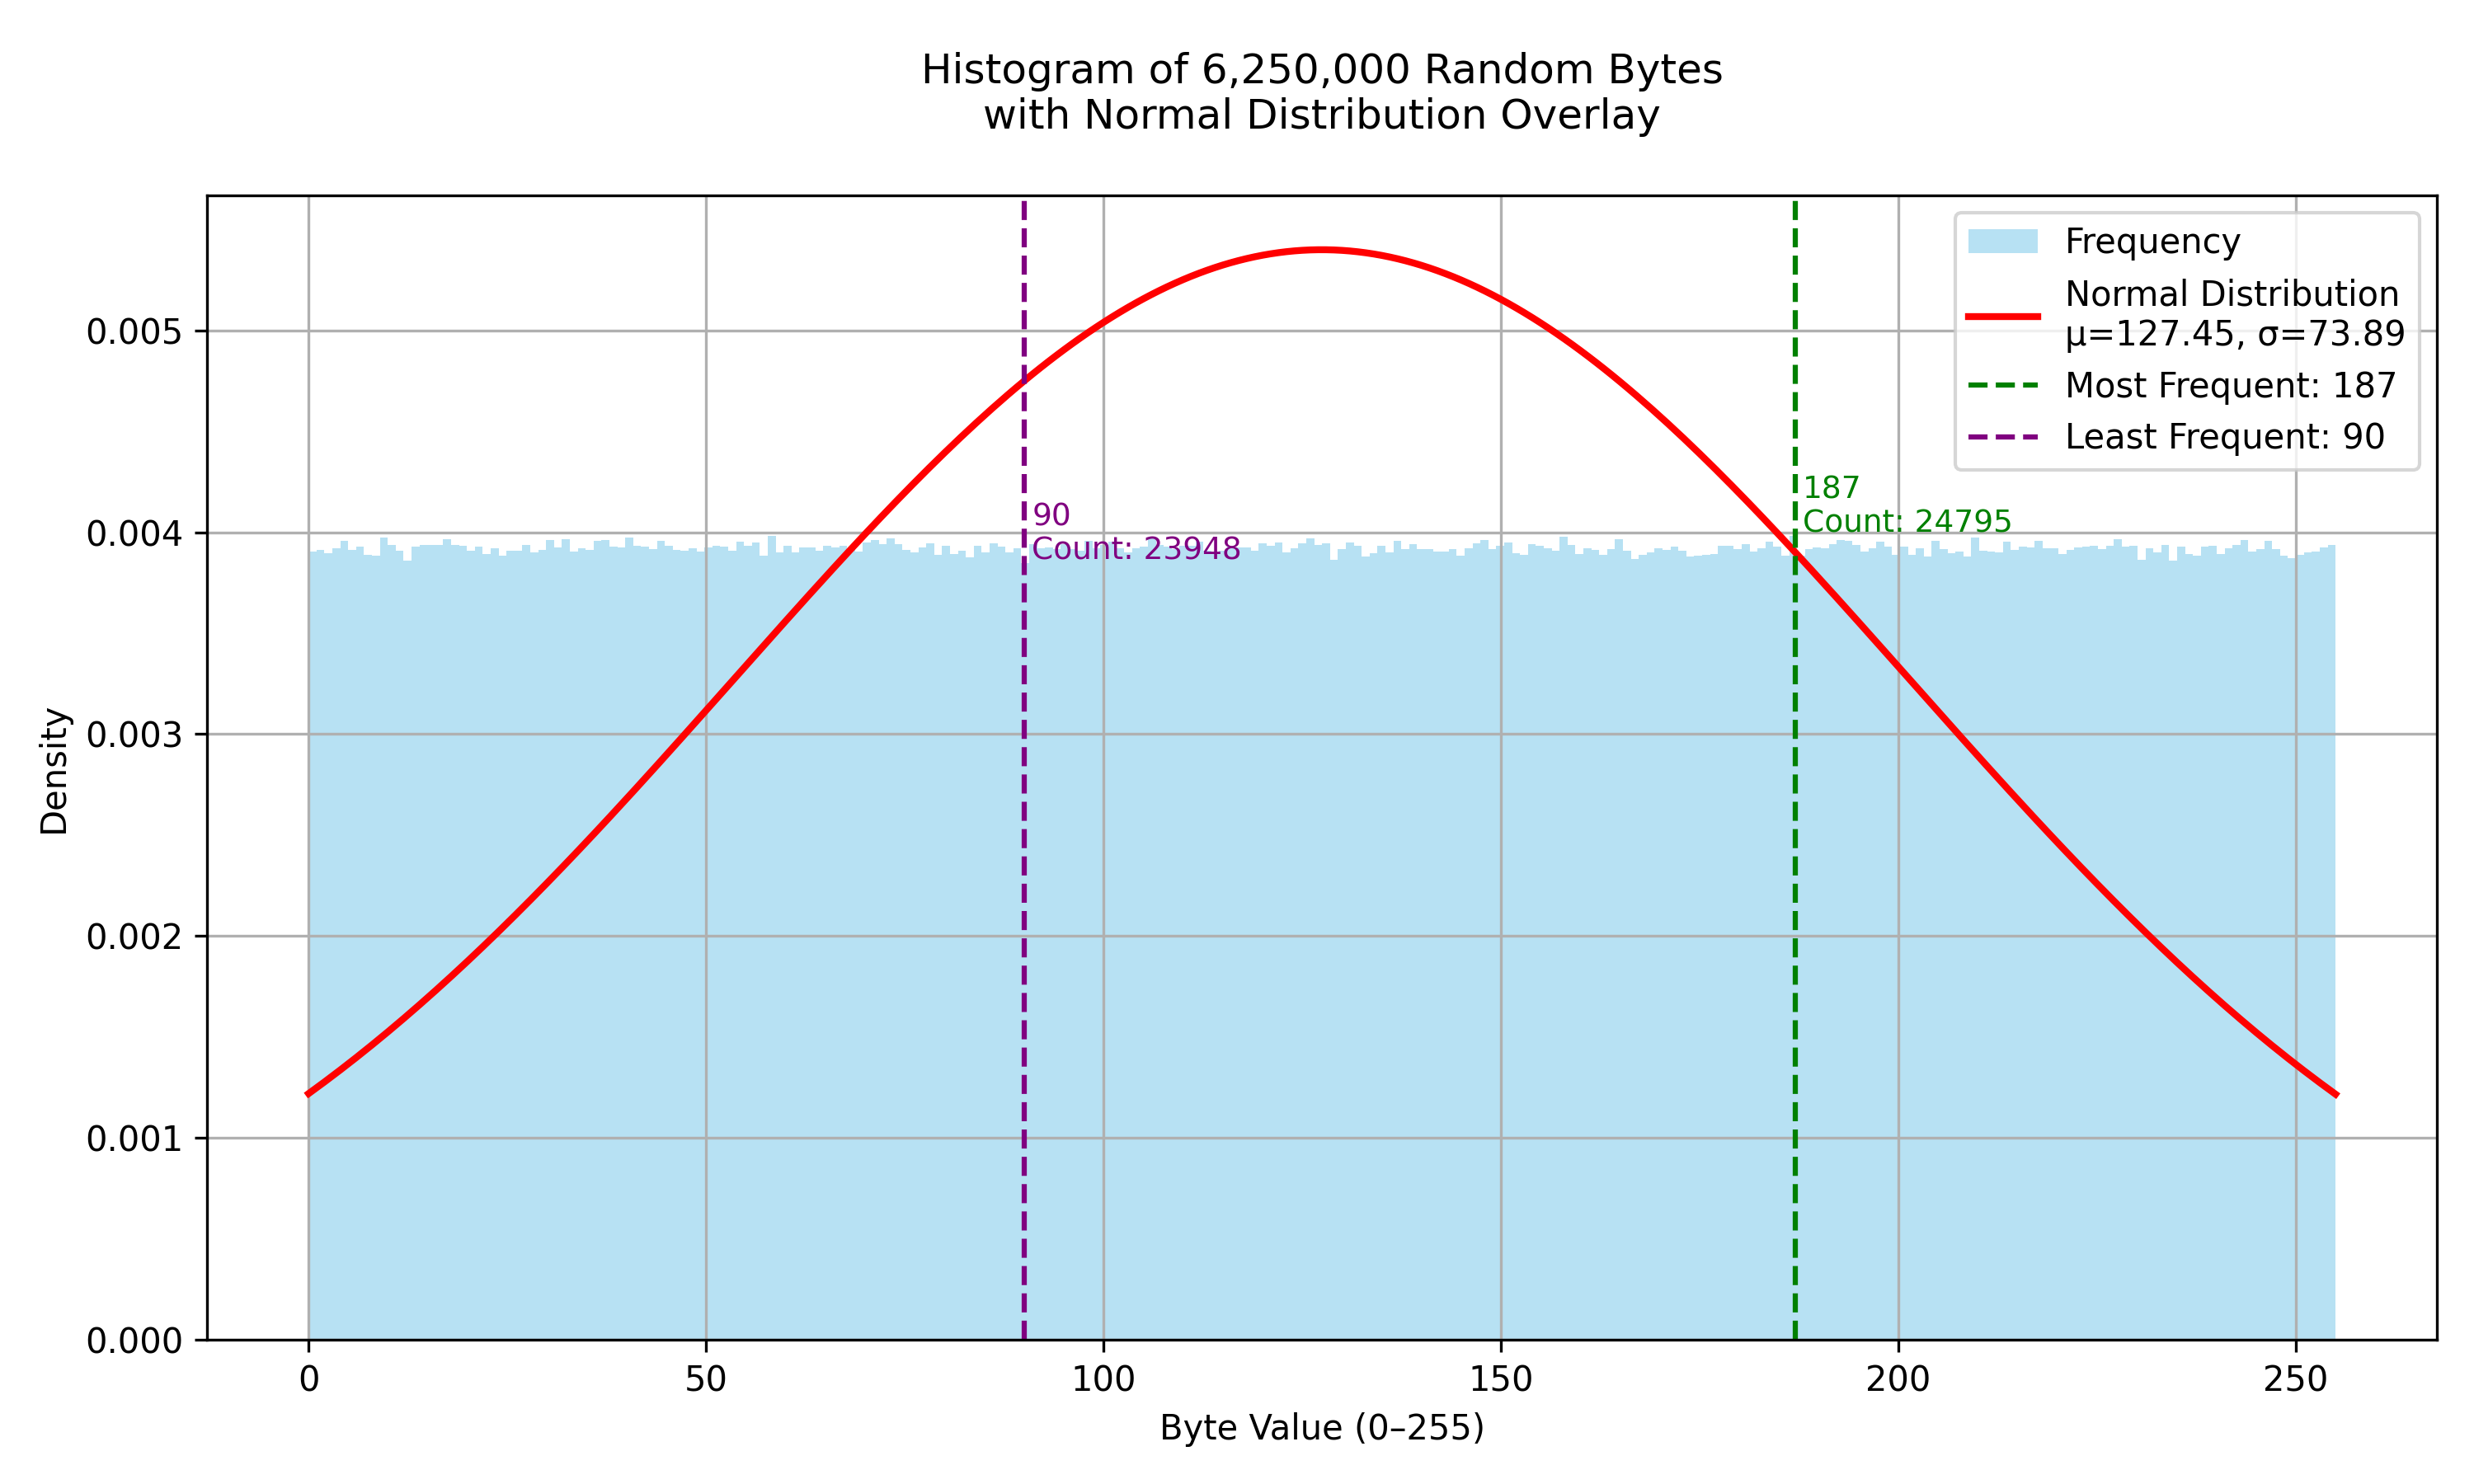
\includegraphics[width=0.9\linewidth]{images/random_bits_CTR_DRBG_seed_python_random.png}
    \caption{\raggedright Random bits \textit{CTR\_DRBG} seed generation with Python random function.}
    \label{fig:ctr_drbg_python_random}
\end{figure}


\subsection{Distribution of Random Bits Generated with Sequential Seeds}
\label{sec:distribution_sequential_seed}

For the following test, sequential seeds were used starting at 1 and reaching 6.5 million in the set of natural numbers. This number was converted to binary and turned into a 32-bit number, then it was used as a seed to generate the distribution with the \textit{CTR\_DRBG} method, showing a uniform distribution without much variation. Unexpectedly, it is seen that the distribution behaves very similar to obtaining reliable seeds with true entropy. Below is the graph.

\begin{figure}[htbp]
    \centering
    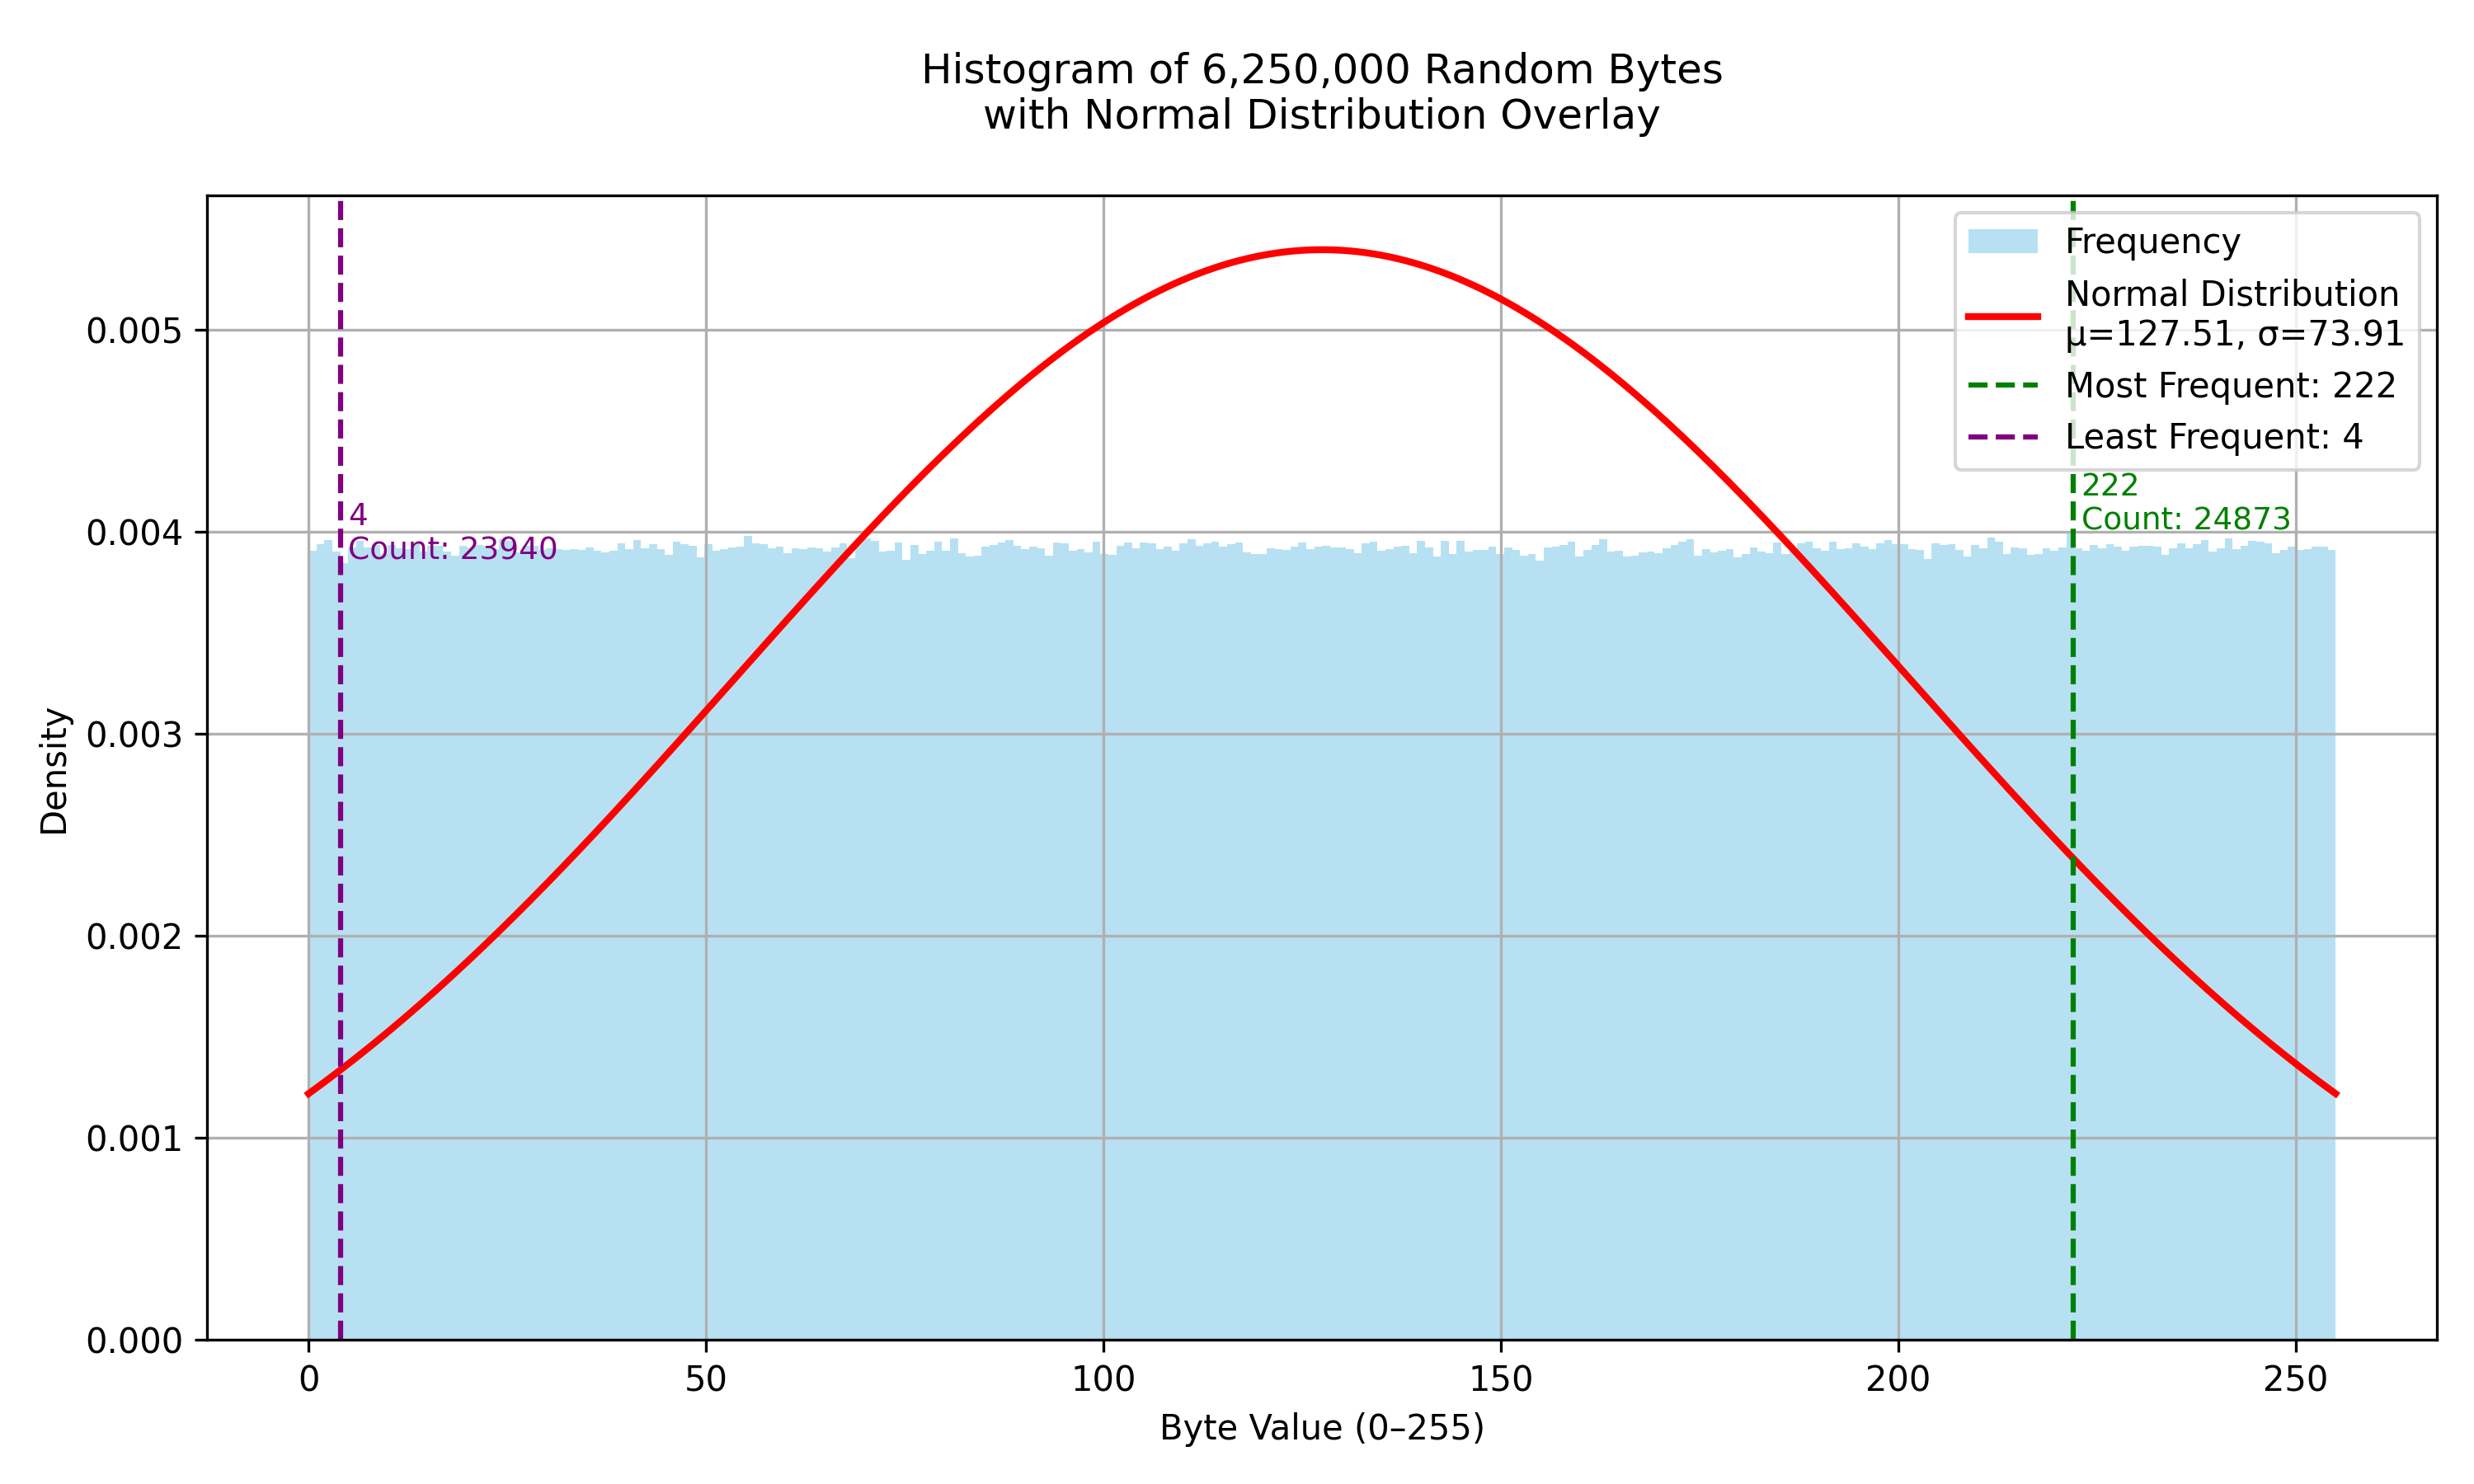
\includegraphics[width=0.9\linewidth]{images/secuentialSeedFrom0_To_100M_CTR_DRBG.png}
    \caption{\raggedright Sequential seed from 1 to 6.5M using \textit{CTR\_DRBG}.}
    \label{fig:ctr_drbg_sequential_seed}
\end{figure}


\section{Conclusions}
The comparative analysis of various random number generators, including classical pseudo-random (CRNG), Counter Mode Deterministic Random Bit Generators (CTR DRBG and CTR DRBG with sequential seeding), and a Quantum Random Number Generator (QRNG), was conducted using a selection of five statistical tests from the NIST SP 800-22 Rev 1a suite. These tests, namely the Frequency (Monobit) Test, Frequency Test within a Block, Runs Test, Maurer's "Universal Statistical" Test, and the Cumulative Sums (Cusum) Test, proved invaluable in assessing different aspects of randomness, from basic bit balance to compressibility and trend analysis . The results indicated that both CTR DRBG implementations exhibited excellent statistical properties, passing all applied tests and demonstrating characteristics consistent with high-quality random data suitable for cryptographic applications. In contrast, the evaluated QRNG, despite its theoretical underpinnings for true randomness, showed significant deviations, failing critical tests such as the Monobit, Runs, and Cusum tests, suggesting underlying biases or issues in the generation or collection process that compromise its statistical randomness for the tested 500,000-bit sequence. The classical RNG served as a baseline and generally performed well.


\bibliographystyle{plainnat}
\bibliography{references}

\end{document}
